%%%%%%%%%%%%%%%%%%%%%%%%%%%%%%%%%%%%%%%%%%%%%%%%%%%%%%%%%%%%%%%%%%%%%%%%%%%
%
% Plantilla para un artículo en LaTeX en español.
%
%%%%%%%%%%%%%%%%%%%%%%%%%%%%%%%%%%%%%%%%%%%%%%%%%%%%%%%%%%%%%%%%%%%%%%%%%%%

\documentclass{article}

% Esto es para poder escribir acentos directamente:
\usepackage[utf8]{inputenc}
% Esto es para que el LaTeX sepa que el texto está en español:
\usepackage[spanish]{babel}
%\usepackage[latin1]{inputenc}

% Paquetes de la AMS:
\usepackage{amsmath, amsthm, amsfonts}

\usepackage{graphicx}

\usepackage{epstopdf}

\usepackage{color}
\usepackage{listings}
\usepackage{setspace}

\textheight=23.94cm
\textwidth=17cm
\topmargin=-1.5cm
\oddsidemargin=0cm
\renewcommand{\baselinestretch}{1.5}
\parindent=0cm 

\definecolor{Code}{rgb}{0,0,0}
\definecolor{Decorators}{rgb}{0.5,0.5,0.5}
\definecolor{Numbers}{rgb}{0.5,0,0}
\definecolor{MatchingBrackets}{rgb}{0.25,0.5,0.5}
\definecolor{Keywords}{rgb}{0,0,1}
\definecolor{self}{rgb}{0,0,0}
\definecolor{Strings}{rgb}{0,0.63,0}
\definecolor{Comments}{rgb}{0,0.63,1}
\definecolor{Backquotes}{rgb}{0,0,0}
\definecolor{Classname}{rgb}{0,0,0}
\definecolor{FunctionName}{rgb}{0,0,0}
\definecolor{Operators}{rgb}{0,0,0}
\definecolor{Background}{rgb}{0.98,0.98,0.98}

\lstnewenvironment{python}[1][]{
\lstset{
numbers=left,
numberstyle=\footnotesize,
numbersep=1em,
xleftmargin=1em,
framextopmargin=2em,
framexbottommargin=2em,
showspaces=false,
showtabs=false,
showstringspaces=false,
frame=l,
tabsize=4,
% Basic
basicstyle=\ttfamily\small\setstretch{1},
backgroundcolor=\color{Background},
language=Python,
% Comments
commentstyle=\color{Comments}\slshape,
% Strings
stringstyle=\color{Strings},
morecomment=[s][\color{Strings}]{"""}{"""},
morecomment=[s][\color{Strings}]{'''}{'''},
% keywords
morekeywords={import,from,class,def,for,while,if,is,in,elif,else,not,and,or,print,break,continue,return,True,False,None,access,as,,del,except,exec,finally,global,import,lambda,pass,print,raise,try,assert},
keywordstyle={\color{Keywords}\bfseries},
% additional keywords
morekeywords={[2]@invariant},
keywordstyle={[2]\color{Decorators}\slshape},
emph={self},
emphstyle={\color{self}\slshape},
%
}}{}


%--------------------------------------------------------------------------
\title{Parcial 2 - Implementación de un codificador y decodificador en lenguaje Python con Spyder}
\author{Jorge Ulises Useche Cuellar\\
  \small Código: 20091005082\\
  \small Ingeniería Electrónica\\
  \small Universidad Distrital\\
  \small 2014-II
}

\begin{document}
\maketitle

\abstract{En este escrito se pretende explicar los algoritmos que se usaron, cómo se grafican datos y los resultados de la codificación de línea Miller.}

\section{Creación de funciones o rutinas recurrentes}

\subsection{Generación de tren de pulsos}

Se crea una función que tiene como parámetros de entrada el tamaño del tren de pulsos y la probabilidad de unos o valores $True$. Para el ejercicio el valor booleano $True$ representará un nivel lógico 1 y el valor $False$ un nivel 0.

\begin{python}
#Generador de tren de pulsos
def flujobinario(tamano,p1):
    c=[]    
    for x in range(0, tamano):
        a = random()
        if(a <= p1):
            b=True
        else:
            b=False
        c.append(b)
    return c
\end{python}

\subsection{Funciones de conversión de valores booleanos a representación binaria con números}

\subsubsection{Conversión de arreglos a booleano}

En esta función se pide un arreglo que solo contenga niveles lógicos y los convierte a valores lógicos.

\begin{python}
#Convertir el arreglo de 1 y 0 a valores booleanos    
def tobool(arreglo):
    c=[]    
    for x in range(0, len(arreglo)):
        if(arreglo[x]==1):
            c.append(True)
        else:
            c.append(False)
    return c
\end{python}

\subsubsection{Conversión a niveles lógicos}

Al igual que el anterior, solo se ingresa un arreglo a la función, pero éste debe contener solo valores lógicos $True$ y $False$, para ser convertido a niveles lógicos 1 y 0.

\begin{python}
#Convertir el arreglo de valores booleanos a 1 y 0
def tonum(arreglo):
    c=[]    
    for x in range(0, len(arreglo)):
        if(arreglo[x]==True):
            c.append(1)
        else:
            c.append(0)
    return c
\end{python}

\subsection{Generación de impulsos de reloj}

Se genera un pulso de reloj que permite al usuario comparar con los tiempos de la señal $a_{k+1}$ o la $Miller$.

\begin{python}
#Genera un pulso entre 0 y 1 alternados
def reloj(tamano):
    tamano=int(tamano)
    c=[]
    p1=True;#porque el primer es not True = False
    for x in range(0, tamano):
        p1 = not p1
        c.append(p1)
    return c
\end{python}

\subsection{Converitur un arreglo para graficar con la función $step$}

La función $step$, nos permite ver los cambios entre niveles con respecto al anterior, es decir, si se tiene en el vector que se va a graficar un 0 y el siguiente valor es un 0, graficará una línea entre esos ceros. Un ejemplo de vector que tendríamos para graficar sería [0,1,0] si se grafica con step, veremos como si el primer valor fuera 1 y luego 0. Es decir, se necesita 1 valor mas de la longitud del arreglo para ver reflejado los valores con el comando $step$. Para este caso, habría que graficar un [0,0,1,0] que es repetir el primer número del arreglo 2 veces y consecuentemente habría que aumentarse el 1, el número de muestras o valores del tiempo discreto, aunque como eso no es tan conveniente para el desarrollo del algoritmo ya que el número de muestras variable complicaría la comprensión del ejercicio. Por esta razón, se suprime el último valor quitando información, pero aumentando la comprensión del mismo. Si no se quisiera perder esta información del último valor, bastaría con aumentar en uno el tamaño del tiempo discreto, realizando los cambios pertinentes en todas las secciones del código donde se haga el llamado al tiempo.

\begin{python}
#Transforma los arreglos para graficar    
def tograph(arreglo):
    arreglo = arreglo[:]
    arreglo.insert(0,arreglo[0])
    arreglo.pop()
    return arreglo
\end{python}

\subsection{Conversión a pulsos simétricos a ceros como una representación de tensión entre +1 y -1 voltios}

Esta función nos convierte un tren de pulsos en una representación numérica que asocia un 0 lógico a un -1 voltios y un 1 lógico a +1 voltios, que son los niveles de voltaje que se envían realmente, buscando no enviar componentes DC en la señal.

\begin{python}
#Trasforma un nivel lo'gico a una se~nal entre
# +V o +1 para True y -V o -1 para False
def tovoltage(arreglo):
    c=[]    
    for x in range(0, len(arreglo)):
        if(arreglo[x]==True):
            c.append(1)
        else:
            c.append(-1)
    return c
\end{python}

\section {Codificador Miller}

Se va a explicar todo el proceso desde la generación del tren de pulsos hasta que se obtiene y gráfica la señal miller.

\subsection {Generación de tren de pulsos aleatorio probabilista}

Para generar la señal $a_{k+a}$ se usa el código:
\begin{python}
ak1=flujobinario(100,0.5)
#ak1=tobool([1,0,0,1,1,0,0,1,0,1])
\end{python}

Se puede ver una línea comentada para el $a_{k+1}$  que nos da un vector de prueba reducido de un ejercicio hecho en clase que nos permite visualizar la veracidad del resultado tanto en vectores como en gráficas.

\subsection{Implementación de máquina de estados}

Como toda máquina debe tener un $``Reset"$, se implementa poniendo el término $ek1$ que representa al $e_{k+1}$ en $True$.

\begin{python}
#reset s0
ek1=[]
ek1.append(True);
\end{python}

Seguido a esto se describe la lógica en cuanto a operadores lógicos para el estado presente y futuro. Como aparecía en la codificación de estados, los bits que nos determinan el estado presente son el $b_{k+1}$ y el $e_{k+1}$, pero a su vez el $b_{k+1}$ es el mismo $a_{k+1}$ y el $e_{k+1}$ es una combinación de terminos presentes ($b_{k}$ y $e_{k}$ )y futuros como se describe:

\begin{python}
bk1=ak1;
for i in range(1, len(ak1)):
    ek1.append(( ak1[i] and (not ek1[i-1]) ) or
        ( (not ak1[i]) and (ak1[i-1] == ek1[i-1]) ))
\end{python}

El valor de $e_{k}$ ha sido reemplazado por $e_{(k+1)-1}$  y no se usa el el valor de $a_{k+1}$ en vez del de $b_{k+1}$ para mostrar a quien lea el código que existe esa igualdad.

\subsection{Generación de CLK's}

Como solo con estos valores de $b_{(k+1)-1}$ y $e_{(k+1)-1}$ no se puede graficar, generamos una base de tiempo entera y divisible por 2 para que haya una correspondencia entre el $CLK$ de periodo $T=100$ y $CLK2$ que es una multiplicación por dos de la frecuencia de $CLK$ y por tanto tiene periodo $T=100/2=50$. La generación de ambos relojes corresponde a una base de tiempo $clkt$ ($t$ de tiempo) y $clk2t$ y a un valor para cada punto de esa base de tiempo, en las variables $clks$ ($s$ de señal) y $clk2s$.

\begin{python}
clkt = range(0,len(ak1)*100,100)
clks = tonum(reloj(len(ak1)))
clk2t = range(0,len(ak1)*100,int(100/2))
clk2s = tonum(reloj(len(ak1)*2))
\end{python}

\subsection{Implementación de la codificación MILLER}

Para generar el pulso de la codificación Miller, se establece una base de tiempo para este y a pesar de que se pudo haber creado una sola base de tiempo para todas las señales, es mas comprensible crear una para cada señal. En este caso es la misma que para el $CLK2$, se hace el vector por medio de los condicionales $if$ y $elif$ y en consola se imprimen los valores.

\begin{python}
#Generacio'n del pulso de codificacio'n miller
millert = range(0,len(ak1)*100,int(100/2))
millers = []
#+v = +1, -v = -1
for i in range(0, len(ak1)):
    # Nos muestra el valor de bk1 y ek1 para
    # rectificar si esta' en el estado correcto
    texto = " "+str(bk1[i])+","+str(ek1[i])
    if   bk1[i] == False and ek1[i] == False:
        millers.append(1)
        millers.append(1)
        print "S3 Sc(t)"+texto
    elif bk1[i] == False and ek1[i] == True:
        millers.append(-1)
        millers.append(-1)
        print "S2 Sd(t)"+texto
    elif bk1[i] == True  and ek1[i] == False:
        millers.append(-1)
        millers.append(1)
        print "S1 Sb(t)"+texto
    elif bk1[i] == True  and ek1[i] == True:
        millers.append(1)
        millers.append(-1)
        print "S0 Sa(t)"+texto
\end{python}

Al hacer la prueba con el vector $a_{k+1}=[1,0,0,1,1,0,0,1,0,1]$ se obtiene el siguiente resultado.

\begin{verbatim}
S0 Sa(t) True,True
S2 Sd(t) False,True
S3 Sc(t) False,False
S0 Sa(t) True,True
S1 Sb(t) True,False
S3 Sc(t) False,False
S2 Sd(t) False,True
S1 Sb(t) True,False
S3 Sc(t) False,False
S0 Sa(t) True,True
\end{verbatim}

\subsection{Gráficas de la codificación de línea Miller}

Para esta parte, se tiene ya la codificación Miller y para visualizar su resultado, lo haremos con el vector de prueba de $a_{k+a}$ que se dijo anteriormente. 

\begin{python}
#Se grafican las se~nales por medio de step
#Algunas veces hay que hacer modificaciones
# breves al arreglo para su correcta visualizacio'n

#Se inicia la figura 1
figure(1)
#Con el comando subplot se grafica la se~nal CLK
#por medio de los vectores clkt y clks
#CLK
subplot(3,1,1)
step(clkt,tograph(clks))
xlim([clkt[0]-10, clkt[len(clkt)-1]-10])
ylim([-0.5, 1.5])
legend(["CLK"])
#a_{k+1}
subplot(3,1,2)
step(clkt,tograph(ak1),'--')
xlim([clk2t[0]-10, clk2t[len(clk2t)-1]-10])
ylim([-0.5, 1.5])
legend(["a_{k+1}"])
#MILLER
subplot(3,1,3)
step(millert,tograph(millers),'--')
xlim([millert[0]-10, millert[len(millert)-1]-10])
ylim([-1.5, 1.5])
legend(["Miller"])

show()
\end{python}

Al ejecutar el código se obtiene el gráfico de la figura \ref{fig:codificadormiller}

\begin{figure}
  \centering
    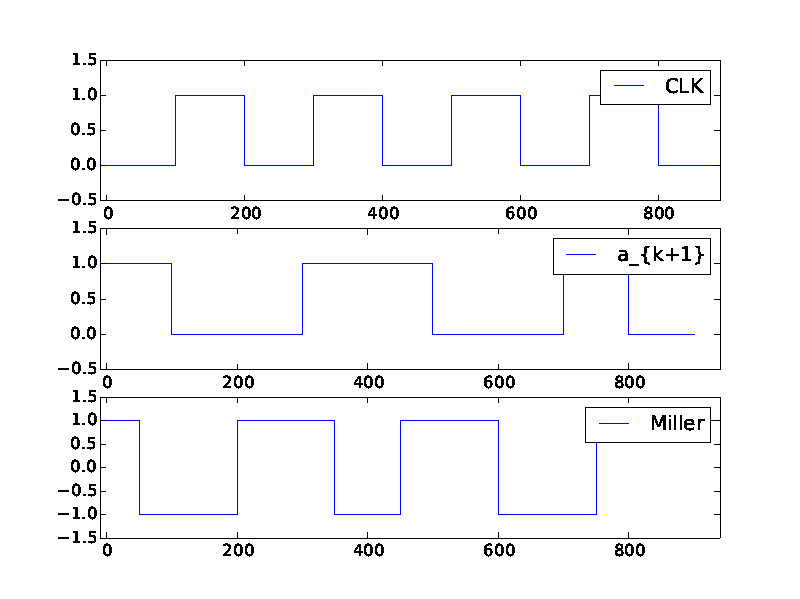
\includegraphics[width=0.95\textwidth]{CodificadorMiller.eps}
  \caption{Codificación Miller}
  \label{fig:codificadormiller}
\end{figure}

\section {Decodificador Miller}

La decodificación se tiene muestreando la señal Miller en los flancos de $CLK2$, como habíamos escrito, el periodo del Miller es igual al del $CLK2$, por tanto se va a muestrear en esos intervalos y se concluye que si los dos valores en ese intervalo son iguales, el mensaje enviado era un 0 o $False$ y si los dos valores de muestra en el intervalo de $CLK$ son diferentes, el mensaje enviado es 1 o $True$.

\begin{python}
#Recuperar ak1
ak1rec=[]
for i in range(0, int(len(millers)/2)):
    if(millers[2*i]==millers[2*i+1]):
        ak1rec.append(False)
    else:
        ak1rec.append(True)

if ak1 == ak1rec:
    print "El mensaje fue recuperado exitosamente."      
else:
    print "El mensaje no fue recuperado con e'xito."
\end{python}

La ejecución del código tiene como salida.

\begin{verbatim}
El mensaje fue recuperado exitosamente.
\end{verbatim}

\subsection {Gráficas del decodificador Miller}

Como nuevamente hay que mostrar las gráficas en donde el mensaje corresponde al tiempo del semiciclo del $CLK$ y el muestreo al tiempo del semiciclo del $CLK2$, se muestran estas señales junto con el mensaje recuperado de la codificación Miller.

\begin{python}
figure(2) 
#CLK
subplot(3,1,1)
step(clkt,tograph(clks))
xlim([clkt[0]-10, clkt[len(clkt)-1]-10])
ylim([-0.5, 1.5])
legend(["CLK"])
#CLK2
subplot(3,1,2)
step(clk2t,tograph(clk2s))
xlim([clk2t[0]-10, clk2t[len(clk2t)-1]-10])
ylim([-0.5, 1.5])
legend(["CLK2"])
#Decodificador MILLER  
subplot(3,1,3)
step(clkt,tograph(ak1rec))
xlim([clkt[0]-10, clkt[len(clkt)-1]-10])
ylim([-0.5, 1.5])
legend(["Recuperado del Miller"])

show()
\end{python}

 Al ejecutar el código se obtiene el gráfico de la figura \ref{fig:decodificadormiller}

\begin{figure}
  \centering
    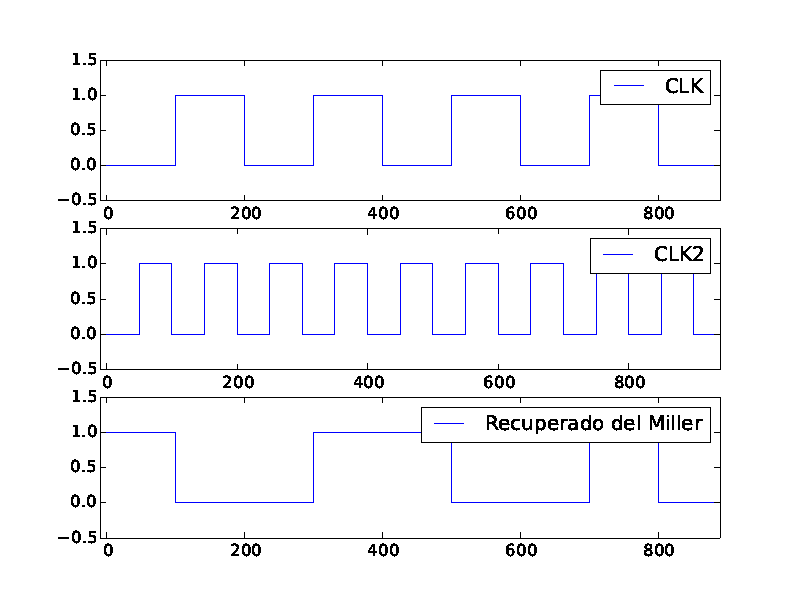
\includegraphics[width=0.95\textwidth]{DecodificadorMiller.eps}
  \caption{Decodificación Miller}
  \label{fig:decodificadormiller}
\end{figure}

\section {Comparación de envío del mensaje sin codificar y codificado}

Como la presencia prolongada de un nivel DC genera un desplazamiento de la línea base, que dificulta al receptor la adecuada decodificación de la información. Es importante comparar este nivel para el ejemplo y luego, realizar una comparación con diferentes mensajes de prueba de gran longitud.

\subsection {Comparación del ejemplo}

Se busca la sumatoria de la señal dividido en el número de términos para hallar el nivel DC.

\begin{verbatim}
>>> sum(tovoltage(ak1))/len(ak1)
0.0
>>> sum(millers)/len(millers)
0.10000000000000001
\end{verbatim}

Para este caso en especial y debido a que la longitud del mensaje es muy pequeña, resulta que la codificación miller fue desventajosa en cuanto al nivel DC, por eso es necesario hacer un mensaje un poco más grande. Para empezar vamos a usar la función $generadoraflujobinario$ con 100 términos y una probabilidad de 1 de 50\%. 

\begin{verbatim}
>>> tonum(ak1)
[0, 1, 1, 1, 1, 1, 1, 0, 1, 0, 1, 0, 0, 1, 1, 1, 0, 0, 1, 1, 1,
 0, 0, 0, 0, 1, 0, 1, 0, 1, 0, 0, 1, 1, 1, 1, 0, 0, 0, 1, 0, 0,
 0, 0, 0, 0, 1, 0, 1, 0, 1, 0, 0, 1, 1, 0, 0, 0, 0, 0, 1, 1, 1,
 0, 1, 0, 1, 1, 0, 1, 0, 1, 1, 1, 1, 1, 1, 0, 0, 0, 0, 0, 1, 1,
 1, 1, 1, 1, 1, 1, 0, 1, 0, 1, 1, 0, 1, 1, 0, 0]
>>> sum(tovoltage(ak1))/len(ak1)
0.059999999999999998
>>> sum(millers)/len(millers)
0.01
\end{verbatim}

Las gráficas arrojadas en esta simulación son las de la  figura \ref{fig:ej1coder}  y  \ref{fig:ej1decoder}.

\begin{figure}
  \centering
    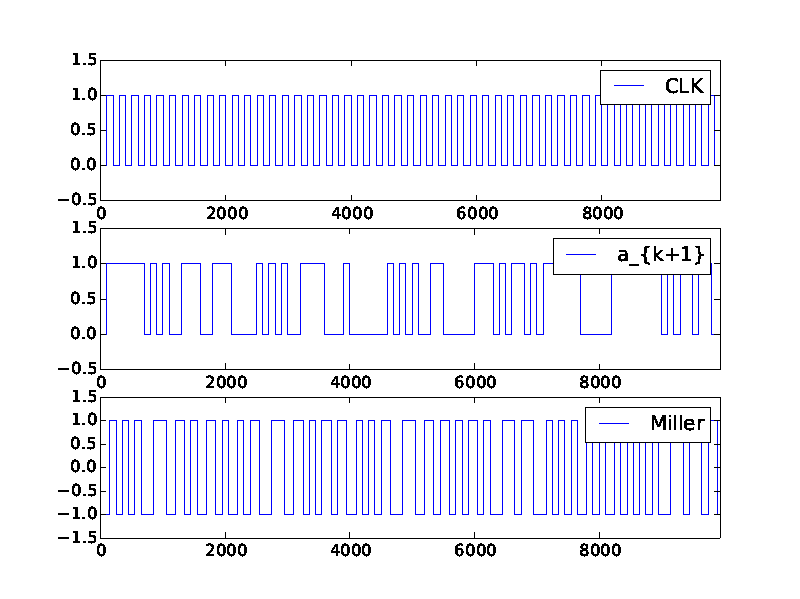
\includegraphics[width=0.95\textwidth]{ej1coder.eps}
  \caption{Codificación Miller 100 bits}
  \label{fig:ej1coder}
\end{figure}

\begin{figure}
  \centering
    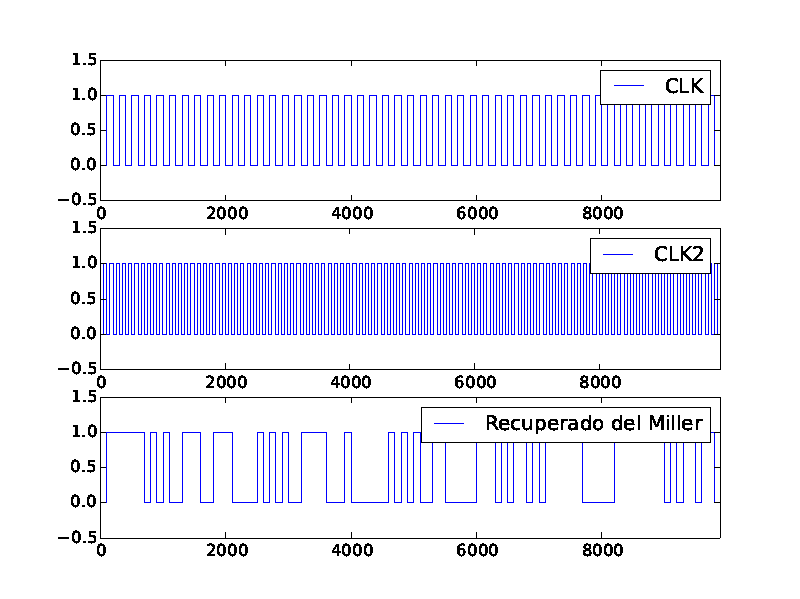
\includegraphics[width=0.95\textwidth]{ej1decoder.eps}
  \caption{Decodificación Miller 100 bits}
  \label{fig:ej1decoder}
\end{figure}

A pesar de que el mensaje tenía una probabilidad del 50\% la codificación Miller ganó esta vez, confirmando la ventaja que tiene la codificación.

De aquí en adelante no mostraremos mas gráficos ya que no se definen los datos, y tampoco se mostrarán los pulsos obtenidos, simplemente los resultados de nivel DC. Para cada uno de las simulaciones se realizó la media de 3 pruebas. Es decir, para la prueba 1 se realizó 3 veces y se ven los resultados.

Se crearon nuevas funciones para este fin:

\begin{python}
def tomiller(ak1):
    #Reset s0
    ek1=[]
    ek1.append(True);
    bk1=ak1;
    for i in range(1, len(ak1)):
        ek1.append(( ak1[i] and (not ek1[i-1]) ) or
            ( (not ak1[i]) and (ak1[i-1] == ek1[i-1]) ))
    
    #Generacio'n del pulso de codificacio'n miller
    millers = []
    #+v = +1, -v = -1
    for i in range(0, len(ak1)):
        if   bk1[i] == False and ek1[i] == False:
            millers.append(1)
            millers.append(1)
        elif bk1[i] == False and ek1[i] == True:
            millers.append(-1)
            millers.append(-1)
        elif bk1[i] == True  and ek1[i] == False:
            millers.append(-1)
            millers.append(1)
        elif bk1[i] == True  and ek1[i] == True:
            millers.append(1)
            millers.append(-1)
    return millers 

def prueba (bits,probabilidad1):
    dcak1prom=0
    dcmillerprom=0
    ak1=flujobinario(bits,probabilidad1)        
    miller=tomiller(ak1)
    dcak1prom=float(sum(tovoltage(ak1)))/len(ak1)
    dcmillerprom=float(sum(miller))/len(miller)
    print " DC del mensaje: "+ str("\%.12f" \% dcak1prom)
    print "DC del miller: "+ str("\%.12f" \% dcmillerprom)
    if abs(dcmillerprom) < abs(dcak1prom):
        print "El valor DC de la codificacion MILLER es la menor" 
\end{python}

Y se ejecutó la prueba:

Para un mensaje de 1000 términos con probabilidad de unos de 50\%
\begin{verbatim}
>>> prueba(1000,0.5)
Dc del mensaje: -0.036000000000
Dc del Miller: 0.002000000000
El DC del miller es menor que la del mensaje
>>> prueba(1000,0.5)
Dc del mensaje: 0.028000000000
Dc del Miller: 0.016000000000
El DC del miller es menor que la del mensaje
>>> prueba(1000,0.5)
Dc del mensaje: 0.004000000000
Dc del Miller: -0.018000000000
\end{verbatim}

Para un mensaje de 1000 términos con probabilidad de unos de 10\%
\begin{verbatim}
>>> prueba(1000,0.1)
Dc del mensaje: -0.788000000000
Dc del Miller: 0.000000000000
El DC del miller es menor que la del mensaje
>>> prueba(1000,0.1)
Dc del mensaje: -0.776000000000
Dc del Miller: 0.008000000000
El DC del miller es menor que la del mensaje
>>> prueba(1000,0.1)
Dc del mensaje: -0.820000000000
Dc del Miller: -0.002000000000
El DC del miller es menor que la del mensaje
\end{verbatim}

Para un mensaje de 1000 términos con probabilidad de unos de 90\%
\begin{verbatim}
>>> prueba(1000,0.9)
Dc del mensaje: 0.810000000000
Dc del Miller: -0.001000000000
El DC del miller es menor que la del mensaje
>>> prueba(1000,0.9)
Dc del mensaje: 0.818000000000
Dc del Miller: -0.001000000000
El DC del miller es menor que la del mensaje
>>> prueba(1000,0.9)
Dc del mensaje: 0.812000000000
Dc del Miller: -0.004000000000
El DC del miller es menor que la del mensaje
\end{verbatim}

Para un mensaje de 10000 términos con probabilidad de unos de 50\%
\begin{verbatim}
>>> prueba(10000,0.5)
Dc del mensaje: -0.006400000000
Dc del Miller: -0.003400000000
El DC del miller es menor que la del mensaje
>>> prueba(10000,0.5)
Dc del mensaje: -0.019400000000
Dc del Miller: -0.002500000000
El DC del miller es menor que la del mensaje
>>> prueba(10000,0.5)
Dc del mensaje: 0.005800000000
Dc del Miller: 0.001300000000
El DC del miller es menor que la del mensaje
\end{verbatim}

Para un mensaje de 10000 términos con probabilidad de unos de 10\%
\begin{verbatim}
>>> prueba(10000,0.1)
Dc del mensaje: -0.807000000000
Dc del Miller: 0.001300000000
El DC del miller es menor que la del mensaje
>>> prueba(10000,0.1)
Dc del mensaje: -0.802000000000
Dc del Miller: -0.000400000000
El DC del miller es menor que la del mensaje
>>> prueba(10000,0.1)
Dc del mensaje: -0.797400000000
Dc del Miller: 0.000700000000
El DC del miller es menor que la del mensaje
\end{verbatim}

Para un mensaje de 1000 términos con probabilidad de unos de 90\%
\begin{verbatim}
>>> prueba(10000,0.9)
Dc del mensaje: 0.800800000000
Dc del Miller: -0.001200000000
El DC del miller es menor que la del mensaje
>>> prueba(10000,0.9)
Dc del mensaje: 0.802600000000
Dc del Miller: -0.001500000000
El DC del miller es menor que la del mensaje
>>> prueba(10000,0.9)
Dc del mensaje: 0.807000000000
Dc del Miller: -0.001500000000
El DC del miller es menor que la del mensaje
\end{verbatim}

\section {Conclusiones}

\begin{itemize}
\item La implementación en un lenguaje de programación hace mas versátil el análisis de la codificación y el análisis numérico del mismo.
\item La codificación Miller puede no suponer la mejor solución entre todas las codificaciones, pero según los datos arrojados si supone una reducción del valor DC de aproximadamente 99.8\% para los 10000 bits, de 94.4\% para 1000 bits y de solo 17\% para el de 100bits. 
\item La codificación para el mensaje de 10 bits no dio resultados muy concluyentes o diferenciales, pero al hacer la prueba más veces en la misma longitud, se nota un poco mas la diferencia, claro está, cuando el nivel DC del mensaje no tiene nivel DC 0, de lo contrario el nivel DC de la codificación Miller, siempre es mayor o igual.
\item Entre mayor es el número de bits del mensaje, mayor es la diferencia entre el valor DC promedio del no codificado y el de codificación Miller.
\end{itemize}

\end{document}